\documentclass{ximera}

%\usepackage{todonotes}

\newcommand{\todo}{}

\usepackage{esint} % for \oiint
\ifxake%%https://math.meta.stackexchange.com/questions/9973/how-do-you-render-a-closed-surface-double-integral
\renewcommand{\oiint}{{\large\bigcirc}\kern-1.56em\iint}
\fi


\graphicspath{
  {./}
  {ximeraTutorial/}
  {basicPhilosophy/}
  {functionsOfSeveralVariables/}
  {normalVectors/}
  {lagrangeMultipliers/}
  {vectorFields/}
  {greensTheorem/}
  {shapeOfThingsToCome/}
  {dotProducts/}
  {partialDerivativesAndTheGradientVector/}
  {../productAndQuotientRules/exercises/}
  {../normalVectors/exercisesParametricPlots/}
  {../continuityOfFunctionsOfSeveralVariables/exercises/}
  {../partialDerivativesAndTheGradientVector/exercises/}
  {../directionalDerivativeAndChainRule/exercises/}
  {../commonCoordinates/exercisesCylindricalCoordinates/}
  {../commonCoordinates/exercisesSphericalCoordinates/}
  {../greensTheorem/exercisesCurlAndLineIntegrals/}
  {../greensTheorem/exercisesDivergenceAndLineIntegrals/}
  {../shapeOfThingsToCome/exercisesDivergenceTheorem/}
  {../greensTheorem/}
  {../shapeOfThingsToCome/}
  {../separableDifferentialEquations/exercises/}
  {vectorFields/}
}

\newcommand{\mooculus}{\textsf{\textbf{MOOC}\textnormal{\textsf{ULUS}}}}

\usepackage{tkz-euclide}
\usepackage{tikz}
\usepackage{tikz-cd}
\usetikzlibrary{arrows}
\tikzset{>=stealth,commutative diagrams/.cd,
  arrow style=tikz,diagrams={>=stealth}} %% cool arrow head
\tikzset{shorten <>/.style={ shorten >=#1, shorten <=#1 } } %% allows shorter vectors

\usetikzlibrary{backgrounds} %% for boxes around graphs
\usetikzlibrary{shapes,positioning}  %% Clouds and stars
\usetikzlibrary{matrix} %% for matrix
\usepgfplotslibrary{polar} %% for polar plots
\usepgfplotslibrary{fillbetween} %% to shade area between curves in TikZ
%\usetkzobj{all}
\usepackage[makeroom]{cancel} %% for strike outs
%\usepackage{mathtools} %% for pretty underbrace % Breaks Ximera
%\usepackage{multicol}
\usepackage{pgffor} %% required for integral for loops



%% http://tex.stackexchange.com/questions/66490/drawing-a-tikz-arc-specifying-the-center
%% Draws beach ball
\tikzset{pics/carc/.style args={#1:#2:#3}{code={\draw[pic actions] (#1:#3) arc(#1:#2:#3);}}}



\usepackage{array}
\setlength{\extrarowheight}{+.1cm}
\newdimen\digitwidth
\settowidth\digitwidth{9}
\def\divrule#1#2{
\noalign{\moveright#1\digitwidth
\vbox{\hrule width#2\digitwidth}}}




% \newcommand{\RR}{\mathbb R}
% \newcommand{\R}{\mathbb R}
% \newcommand{\N}{\mathbb N}
% \newcommand{\Z}{\mathbb Z}

\newcommand{\sagemath}{\textsf{SageMath}}


%\renewcommand{\d}{\,d\!}
%\renewcommand{\d}{\mathop{}\!d}
%\newcommand{\dd}[2][]{\frac{\d #1}{\d #2}}
%\newcommand{\pp}[2][]{\frac{\partial #1}{\partial #2}}
% \renewcommand{\l}{\ell}
%\newcommand{\ddx}{\frac{d}{\d x}}

% \newcommand{\zeroOverZero}{\ensuremath{\boldsymbol{\tfrac{0}{0}}}}
%\newcommand{\inftyOverInfty}{\ensuremath{\boldsymbol{\tfrac{\infty}{\infty}}}}
%\newcommand{\zeroOverInfty}{\ensuremath{\boldsymbol{\tfrac{0}{\infty}}}}
%\newcommand{\zeroTimesInfty}{\ensuremath{\small\boldsymbol{0\cdot \infty}}}
%\newcommand{\inftyMinusInfty}{\ensuremath{\small\boldsymbol{\infty - \infty}}}
%\newcommand{\oneToInfty}{\ensuremath{\boldsymbol{1^\infty}}}
%\newcommand{\zeroToZero}{\ensuremath{\boldsymbol{0^0}}}
%\newcommand{\inftyToZero}{\ensuremath{\boldsymbol{\infty^0}}}



% \newcommand{\numOverZero}{\ensuremath{\boldsymbol{\tfrac{\#}{0}}}}
% \newcommand{\dfn}{\textbf}
% \newcommand{\unit}{\,\mathrm}
% \newcommand{\unit}{\mathop{}\!\mathrm}
% \newcommand{\eval}[1]{\bigg[ #1 \bigg]}
% \newcommand{\seq}[1]{\left( #1 \right)}
% \renewcommand{\epsilon}{\varepsilon}
% \renewcommand{\phi}{\varphi}


% \renewcommand{\iff}{\Leftrightarrow}

% \DeclareMathOperator{\arccot}{arccot}
% \DeclareMathOperator{\arcsec}{arcsec}
% \DeclareMathOperator{\arccsc}{arccsc}
% \DeclareMathOperator{\si}{Si}
% \DeclareMathOperator{\scal}{scal}
% \DeclareMathOperator{\sign}{sign}


%% \newcommand{\tightoverset}[2]{% for arrow vec
%%   \mathop{#2}\limits^{\vbox to -.5ex{\kern-0.75ex\hbox{$#1$}\vss}}}
% \newcommand{\arrowvec}[1]{{\overset{\rightharpoonup}{#1}}}
% \renewcommand{\vec}[1]{\arrowvec{\mathbf{#1}}}
% \renewcommand{\vec}[1]{{\overset{\boldsymbol{\rightharpoonup}}{\mathbf{#1}}}}

% \newcommand{\point}[1]{\left(#1\right)} %this allows \vector{ to be changed to \vector{ with a quick find and replace
% \newcommand{\pt}[1]{\mathbf{#1}} %this allows \vec{ to be changed to \vec{ with a quick find and replace
% \newcommand{\Lim}[2]{\lim_{\point{#1} \to \point{#2}}} %Bart, I changed this to point since I want to use it.  It runs through both of the exercise and exerciseE files in limits section, which is why it was in each document to start with.

% \DeclareMathOperator{\proj}{\mathbf{proj}}
% \newcommand{\veci}{{\boldsymbol{\hat{\imath}}}}
% \newcommand{\vecj}{{\boldsymbol{\hat{\jmath}}}}
% \newcommand{\veck}{{\boldsymbol{\hat{k}}}}
% \newcommand{\vecl}{\vec{\boldsymbol{\l}}}
% \newcommand{\uvec}[1]{\mathbf{\hat{#1}}}
% \newcommand{\utan}{\mathbf{\hat{t}}}
% \newcommand{\unormal}{\mathbf{\hat{n}}}
% \newcommand{\ubinormal}{\mathbf{\hat{b}}}

% \newcommand{\dotp}{\bullet}
% \newcommand{\cross}{\boldsymbol\times}
% \newcommand{\grad}{\boldsymbol\nabla}
% \newcommand{\divergence}{\grad\dotp}
% \newcommand{\curl}{\grad\cross}
%\DeclareMathOperator{\divergence}{divergence}
%\DeclareMathOperator{\curl}[1]{\grad\cross #1}
% \newcommand{\lto}{\mathop{\longrightarrow\,}\limits}

% \renewcommand{\bar}{\overline}

\colorlet{textColor}{black}
\colorlet{background}{white}
\colorlet{penColor}{blue!50!black} % Color of a curve in a plot
\colorlet{penColor2}{red!50!black}% Color of a curve in a plot
\colorlet{penColor3}{red!50!blue} % Color of a curve in a plot
\colorlet{penColor4}{green!50!black} % Color of a curve in a plot
\colorlet{penColor5}{orange!80!black} % Color of a curve in a plot
\colorlet{penColor6}{yellow!70!black} % Color of a curve in a plot
\colorlet{fill1}{penColor!20} % Color of fill in a plot
\colorlet{fill2}{penColor2!20} % Color of fill in a plot
\colorlet{fillp}{fill1} % Color of positive area
\colorlet{filln}{penColor2!20} % Color of negative area
\colorlet{fill3}{penColor3!20} % Fill
\colorlet{fill4}{penColor4!20} % Fill
\colorlet{fill5}{penColor5!20} % Fill
\colorlet{gridColor}{gray!50} % Color of grid in a plot

\newcommand{\surfaceColor}{violet}
\newcommand{\surfaceColorTwo}{redyellow}
\newcommand{\sliceColor}{greenyellow}




\pgfmathdeclarefunction{gauss}{2}{% gives gaussian
  \pgfmathparse{1/(#2*sqrt(2*pi))*exp(-((x-#1)^2)/(2*#2^2))}%
}


%%%%%%%%%%%%%
%% Vectors
%%%%%%%%%%%%%

%% Simple horiz vectors
\renewcommand{\vector}[1]{\left\langle #1\right\rangle}


%% %% Complex Horiz Vectors with angle brackets
%% \makeatletter
%% \renewcommand{\vector}[2][ , ]{\left\langle%
%%   \def\nextitem{\def\nextitem{#1}}%
%%   \@for \el:=#2\do{\nextitem\el}\right\rangle%
%% }
%% \makeatother

%% %% Vertical Vectors
%% \def\vector#1{\begin{bmatrix}\vecListA#1,,\end{bmatrix}}
%% \def\vecListA#1,{\if,#1,\else #1\cr \expandafter \vecListA \fi}

%%%%%%%%%%%%%
%% End of vectors
%%%%%%%%%%%%%

%\newcommand{\fullwidth}{}
%\newcommand{\normalwidth}{}



%% makes a snazzy t-chart for evaluating functions
%\newenvironment{tchart}{\rowcolors{2}{}{background!90!textColor}\array}{\endarray}

%%This is to help with formatting on future title pages.
\newenvironment{sectionOutcomes}{}{}



%% Flowchart stuff
%\tikzstyle{startstop} = [rectangle, rounded corners, minimum width=3cm, minimum height=1cm,text centered, draw=black]
%\tikzstyle{question} = [rectangle, minimum width=3cm, minimum height=1cm, text centered, draw=black]
%\tikzstyle{decision} = [trapezium, trapezium left angle=70, trapezium right angle=110, minimum width=3cm, minimum height=1cm, text centered, draw=black]
%\tikzstyle{question} = [rectangle, rounded corners, minimum width=3cm, minimum height=1cm,text centered, draw=black]
%\tikzstyle{process} = [rectangle, minimum width=3cm, minimum height=1cm, text centered, draw=black]
%\tikzstyle{decision} = [trapezium, trapezium left angle=70, trapezium right angle=110, minimum width=3cm, minimum height=1cm, text centered, draw=black]


\title{Abs. Value Analysis}

\begin{document}

\begin{abstract}
examples
\end{abstract}
\maketitle









We are building a library of the elemntary functions.  The idea is to use the library to list characteristics, features, and aspects of all functions within each category.  \\

That way, if we can identify the type of function we have, then we get free information when analyzing functions. \\

The category becomes our reasoning. \\



\begin{center}

\textbf{\textcolor{red!70!black}{These are ``CAN'' questions.}} \\

\end{center}




\textbf{\textcolor{purple!85!blue}{CAN}}the formula we are given be rewritten as one of the official standard forms for each category? \\











\begin{formula} \textbf{\textcolor{green!50!black}{Absolute Functions}}

Absolute functions are those functions that \textbf{\textcolor{purple!85!blue}{can}} be represented by formulas of the form


\[      AV(x) = A \cdot | B \, x + C| + D   \]

where $A$, $B$, $C$, and $D$ are real numbers, with $A \ne B$ and $B \ne 0$ is a nonzero real number.


\end{formula}


\textbf{Note:}  In the template for absolute value functions, There is a leading coefficient for the function and there is a leading coefficient for the linear function inside the absolute value bars. \\













\begin{example}

Comnpletely (Algebraically) analyze

\[
T(k) = -3 | 2 - k | + 5
\]









\textbf{\textcolor{blue!55!black}{$\blacktriangleright$ Category}} \\



$T(k) = -3 | 2 - k | + 5$ matches our official template, $A \cdot | B \, x + C| + D$, which makes it an absolute value function.  





\textbf{\textcolor{blue!55!black}{$\blacktriangleright$ Domain}} \\


$T(k))$ is an absolute value function, which means its natural domain is all real numbers, $(-\infty, \infty)$. \\






\textbf{\textcolor{blue!55!black}{$\blacktriangleright$ Zeros}} \\

\[
T(k) = -3 | 2 - k | + 5 = 0
\]

\begin{align*}
-3 | 2 - k | + 5 &= 0 \\
| 2 - k | &= \frac{5}{3} 
\end{align*}


Either,


\begin{align*}
2 - k &= \frac{5}{3} \\
2 - \frac{5}{3} &= k \\ 
\frac{1}{3} &= k 
\end{align*}


Or, 


Either,


\begin{align*}
2 - k &= -\frac{5}{3} \\
2 + \frac{5}{3} &= k \\ 
\frac{11}{3} &= k 
\end{align*}


Two zeros: $\frac{1}{3}$ or $\frac{11}{3}$. \\
















\textbf{\textcolor{blue!55!black}{$\blacktriangleright$ Continuity}} \\

$T$ is continuous, since it is an absolute value function. \\






\textbf{\textcolor{blue!55!black}{$\blacktriangleright$ End-Behavior}} \\


The leading coefficient of $T$ is $-3 < 0$, therefore $T$ goes unbounded negatively. \\


\[
\lim\limits_{k \to -\infty} T(k) = -\infty
\]




\[
\lim\limits_{k \to \infty} T(k) = -\infty
\]









\textbf{\textcolor{blue!55!black}{$\blacktriangleright$ Behavior}} \\


The leading coefficient of $T$ is $-3 < 0$, therefore $T$ increases and then decreases, changing at the critical number. \\


The critical number is the real number that makes the inside equal to $0$. \


$2 - k = 0$ at $k + 2$ \\


$T$ is increasing on $(-\infty, 2)$ and decreasing on $(2, \infty)$. \\


\textbf{Note:}  It is more accurate to say $T$ is increasing on $(-\infty, 2]$ and decreasing on $[2, \infty)$.









\textbf{\textcolor{blue!55!black}{$\blacktriangleright$ Global Maximum and Minimum}} \\


Since $T$ is continuous and increases and then decreases, there is a global maximum of $T(2) = 5$ at $2$.



The end-behaviore tells us that there is no global minimum.








\textbf{\textcolor{blue!55!black}{$\blacktriangleright$ Local Maximum and Minimum}} \\



As an absolute value function, $T$ has a single local maximum or minimum, which is the same as the global maximum or minimum. \\

Therefore, the only local maximum is $5$, which occurs at $2$ \\





\textbf{\textcolor{blue!55!black}{$\blacktriangleright$ Range}} \\


\begin{itemize}
\item $T$ is continuous
\item $\lim\limits_{k \to -\infty} T(k) = -\infty$
\item The global maximum is $5$
\end{itemize}


The range of $T$ is $(-\infty, 5]$










\textbf{\textcolor{blue!55!black}{$\blacktriangleright$ Graph}} \\




The graph of $y = T(k) = -3 | 2 - k | + 5$


\begin{image}
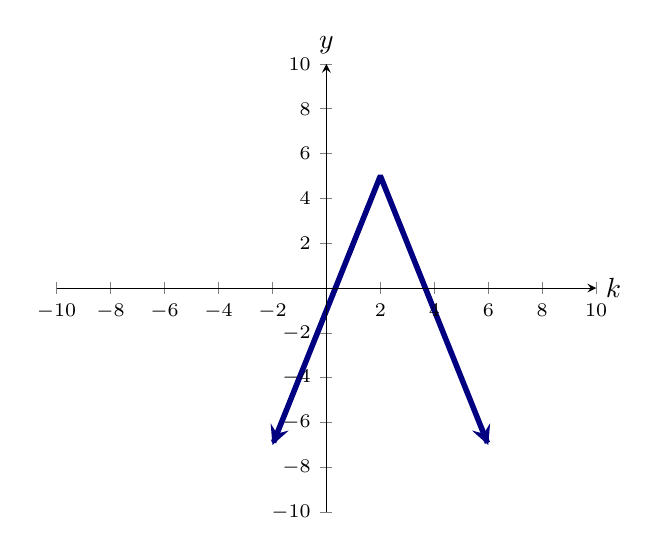
\begin{tikzpicture} 
  \begin{axis}[
            domain=-10:10, ymax=10, xmax=10, ymin=-10, xmin=-10,
            axis lines =center, xlabel=$k$, ylabel=$y$,
            ytick={-10,-8,-6,-4,-2,2,4,6,8,10},
            xtick={-10,-8,-6,-4,-2,2,4,6,8,10},
            ticklabel style={font=\scriptsize},
            every axis y label/.style={at=(current axis.above origin),anchor=south},
            every axis x label/.style={at=(current axis.right of origin),anchor=west},
            axis on top
          ]
          
          	%\addplot [line width=2, penColor, smooth, domain=(-9:0),<->] {(x-1)/((x+3)*(x-4))};
          	\addplot [line width=2, penColor, smooth, samples=200,domain=(-2:6),<->] {-3*abs(2-x)+5};
   
 			%\addplot[color=penColor,fill=penColor,only marks,mark=*] coordinates{(2.5,4)};

           

  \end{axis}
\end{tikzpicture}
\end{image}





\begin{center}
\desmos{bkd48ytcey}{400}{300}
\end{center}


\end{example}























































\begin{center}
\textbf{\textcolor{green!50!black}{ooooo-=-=-=-ooOoo-=-=-=-ooooo}} \\

more examples can be found by following this link\\ \link[More Examples of Analysis]{https://ximera.osu.edu/csccmathematics/precalculus/precalculus/radicalFunctions/examples/exampleList}

\end{center}






\end{document}
